% !TEX root = ../main.tex
\section{Omniglot Dataset Details}
We used the following split details for experiments on Omniglot dataset. This is the same train/test split as \citep{vinyals2016matchingnet}, but we created our own validation split for selecting hyper-parameters. Models are trained on the train split only.

\textbf{Train Alphabets:}
Alphabet\_of\_the\_Magi,
Angelic,
Anglo-Saxon\_Futhorc,
Arcadian,
Asomtavruli\_(Georgian),
Atemayar\_Qelisayer,
Atlantean,
Aurek-Besh,
Avesta,
Balinese,
Blackfoot\_(Canadian\_Aboriginal\_Syllabics),
Braille,
Burmese\_(Myanmar),
Cyrillic,
Futurama,
Ge\_ez,
Glagolitic,
Grantha,
Greek,
Gujarati,
Gurmukhi (character 01-41),
Inuktitut\_(Canadian\_Aboriginal\_Syllabics),
Japanese\_(hiragana),
Japanese\_(katakana),
Korean,
Latin,
Malay\_(Jawi\_-\_Arabic),
N\_Ko,
Ojibwe\_(Canadian\_Aboriginal\_Syllabics),
Sanskrit,
Syriac\_(Estrangelo),
Tagalog,
Tifinagh

\textbf{Validation Alphabets:}
Armenian, 
Bengali, 
Early\_Aramaic, 
Hebrew, 
Mkhedruli\_(Geogian) 

\textbf{Test Alphabets:}
Gurmukhi (character 42-45),
Kannada,
Keble,
Malayalam,
Manipuri,
Mongolian,
Old\_Church\_Slavonic\_(Cyrillic),
Oriya,
Sylheti,
Syriac\_(Serto),
Tengwar,
Tibetan,
ULOG

\section{\textit{tiered}Imagenet Dataset Details}

Each high-level category in \textit{tiered}ImageNet contains between 10 and 30 ILSVRC-12 classes (17.8 on average). In the ImageNet hierarchy, some classes have multiple parent nodes. Therefore, classes belonging to more than one category were removed from the dataset to ensure separation between training and test categories. Test
categories were chosen to reflect various levels of separation between training
and test classes. Some test categories (such as ``working dog'') are fairly similar to training categories, whereas others (such as ``geological formation'')
are quite different. The list of categories is shown below and statistics of the dataset can be found in Table~\ref{tab:tiered_stats}. A visualization of the categories according to the ImageNet hierarchy is shown in Figure~\ref{fig:tiered_hierarchy}. The full list of classes per category will
also be made public, however for the sake of brevity we do not include it here.

\begin{table}[ht]
    \center
    \caption{Statistics of the \textit{tiered}ImageNet dataset.}
    \label{tab:tiered_stats}
    \begin{tabular}{l|cccc}
                   & Train   & Val & Test    & Total \\ \hline
        Categories & 20      & 6   & 8       & 34 \\
        Classes    & 351     & 97  & 160     & 608 \\
        Images     & 448,695 & 124,261   & 206,209 & 779,165 \\
    \end{tabular}
\end{table}

\textbf{Train Categories}:  
\texttt{n02087551} (hound, hound dog), 
\texttt{n02092468} (terrier),  
\texttt{n02120997} (feline, felid),  
\texttt{n02370806} (ungulate, hoofed mammal),
\texttt{n02469914} (primate),  
\texttt{n01726692} (snake, serpent, ophidian),  
\texttt{n01674216} (saurian),
\texttt{n01524359} (passerine, passeriform bird),  
\texttt{n01844917} (aquatic bird),  
\texttt{n04081844} (restraint, constraint),  
\texttt{n03574816} (instrument),  
\texttt{n03800933} (musical instrument, instrument),  
\texttt{n03125870} (craft),
\texttt{n04451818} (tool),  
\texttt{n03414162} (game equipment),
\texttt{n03278248} (electronic equipment),  
\texttt{n03419014} (garment), 
\texttt{n03297735} (establishment), 
\texttt{n02913152} (building, edifice),
\texttt{n04014297} (protective covering, protective cover, protection).

\textbf{Validation Categories}: 
\texttt{n02098550} (sporting dog, gun dog),
\texttt{n03257877} (durables, durable goods, consumer durables),
\texttt{n03405265} (furnishing),
\texttt{n03699975} (machine),  
\texttt{n03738472} (mechanism),
\texttt{n03791235} (motor vehicle, automotive vehicle), 


\textbf{Test Categories}: \texttt{n02103406} (working dog),  \texttt{n01473806} (aquatic vertebrate),
\texttt{n02159955} (insect), \texttt{n04531098} (vessel),
\texttt{n03839993} (obstruction, obstructor, obstructer, impediment, impedimenta),
\texttt{n09287968} (geological formation, formation), \texttt{n00020090} (substance),  \texttt{n15046900} (solid).


\iflatexml
\begin{figure}[ht]
    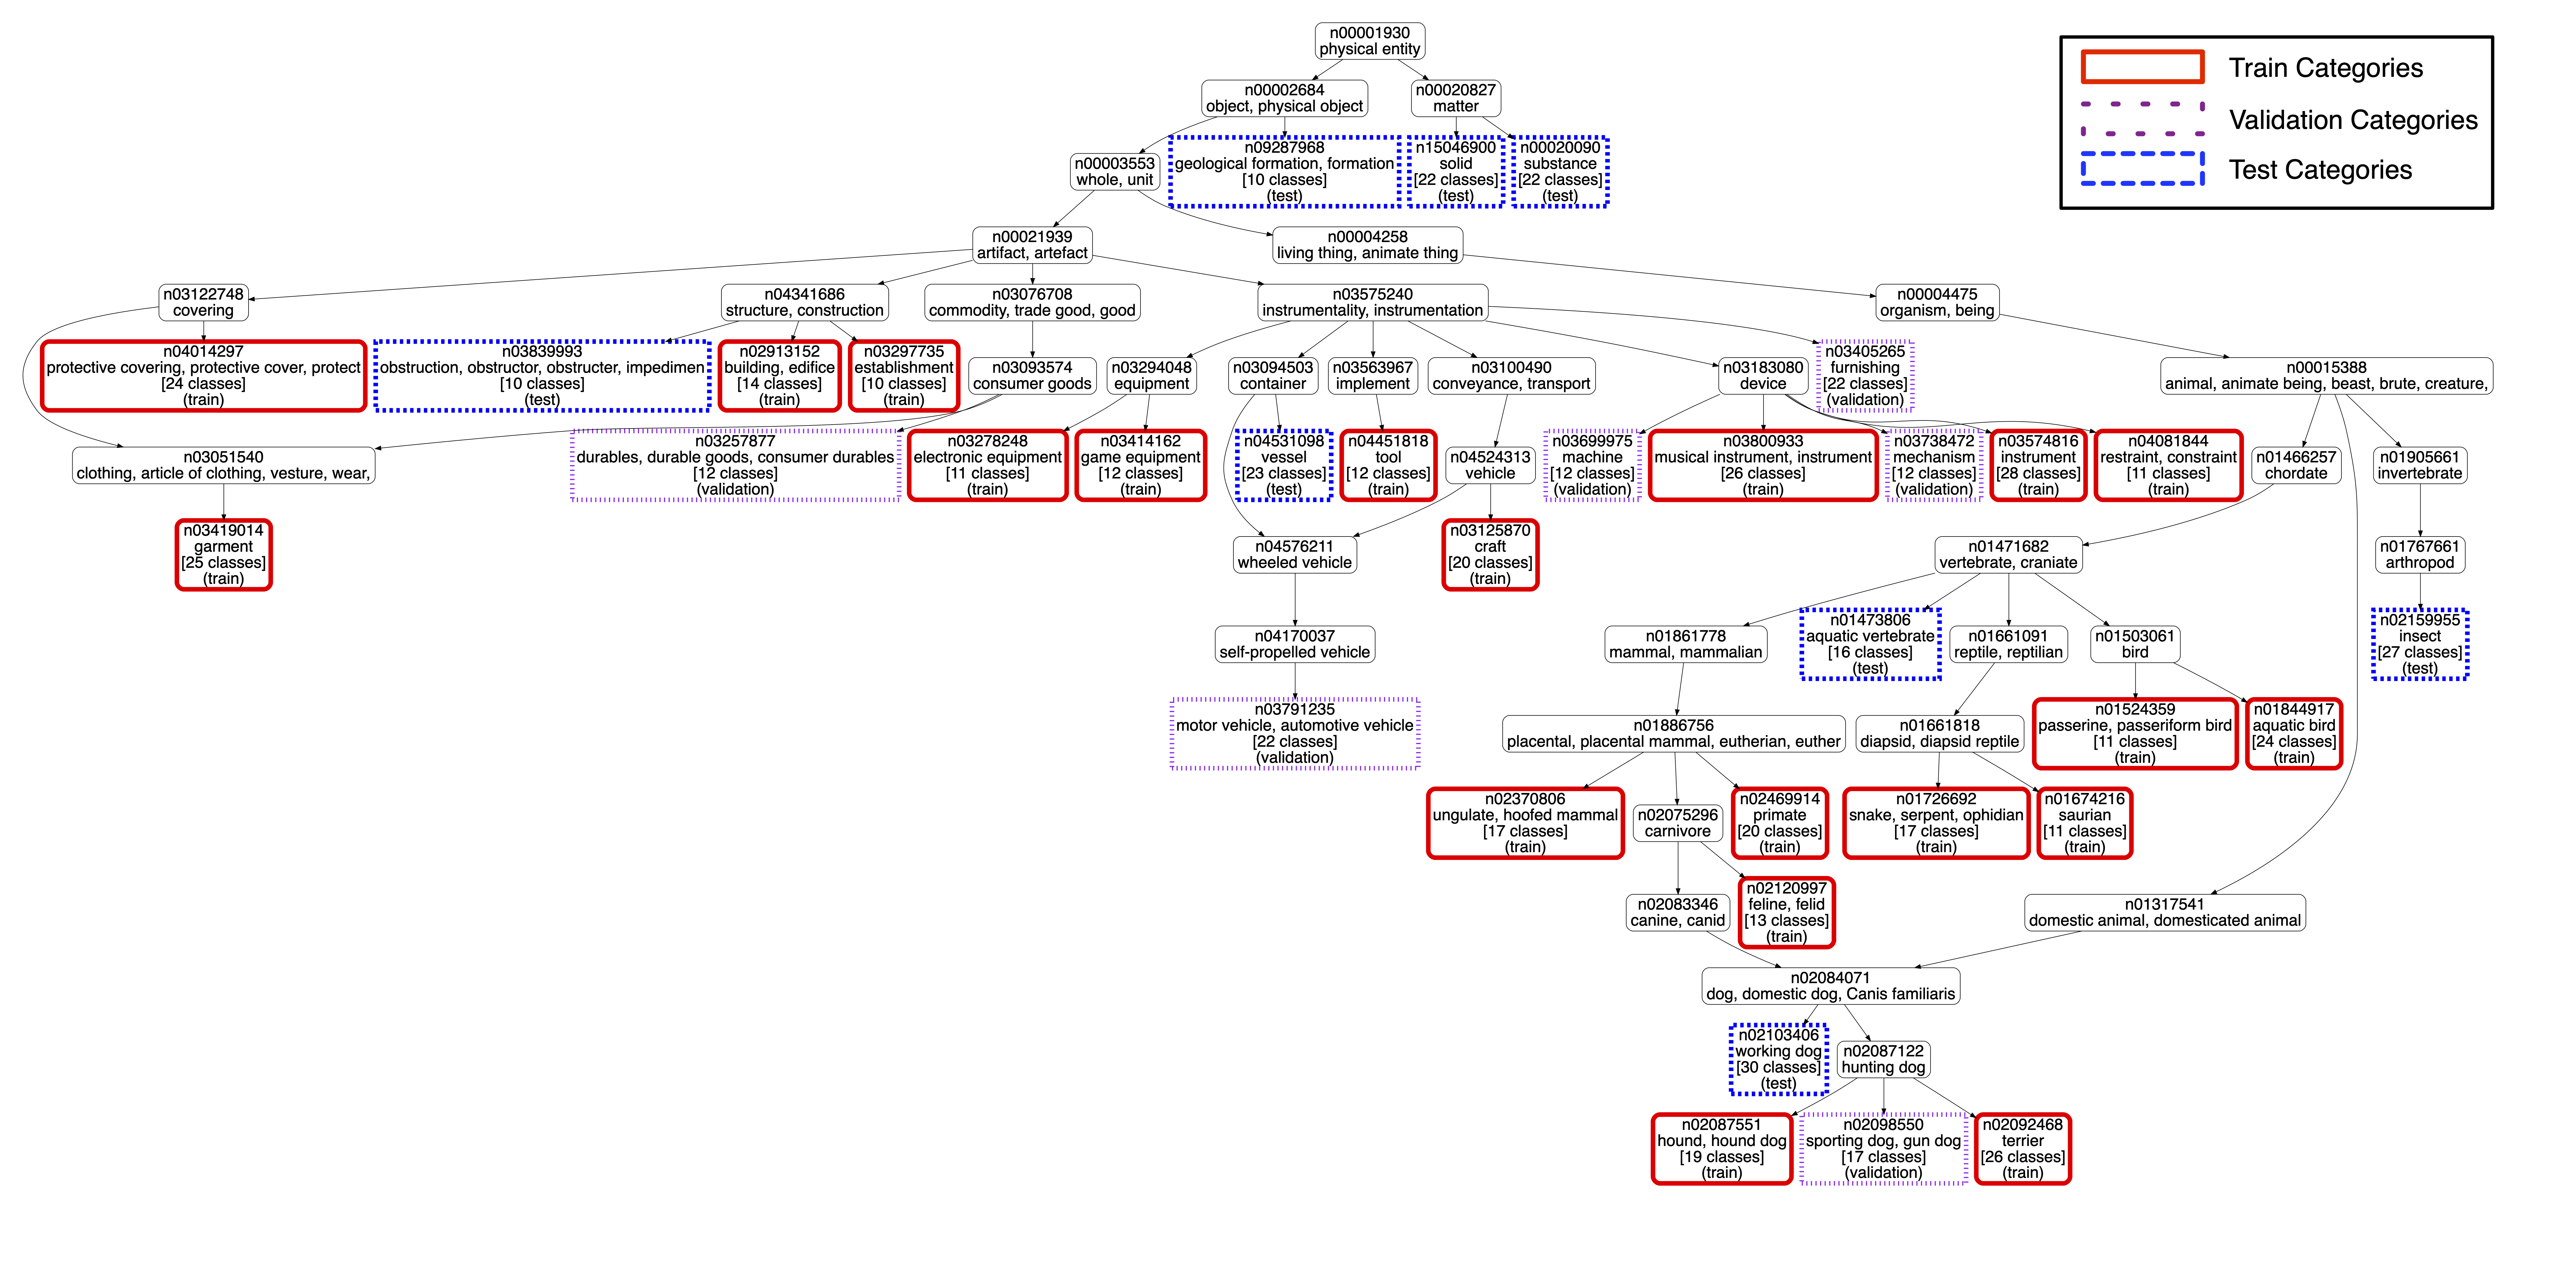
\includegraphics[width=8\textwidth]{figures/hierarchy_legend_val.png}
    \caption{Hierarchy of \textit{tiered}Imagenet categories. Training categories are highlighted in red and test categories in blue. Each category indicates the number of associated classes from ILSVRC-12. Best viewed zoomed-in on electronic version.}
    \label{fig:tiered_hierarchy}
\end{figure}
\else
\begin{sidewaysfigure}[ht]
    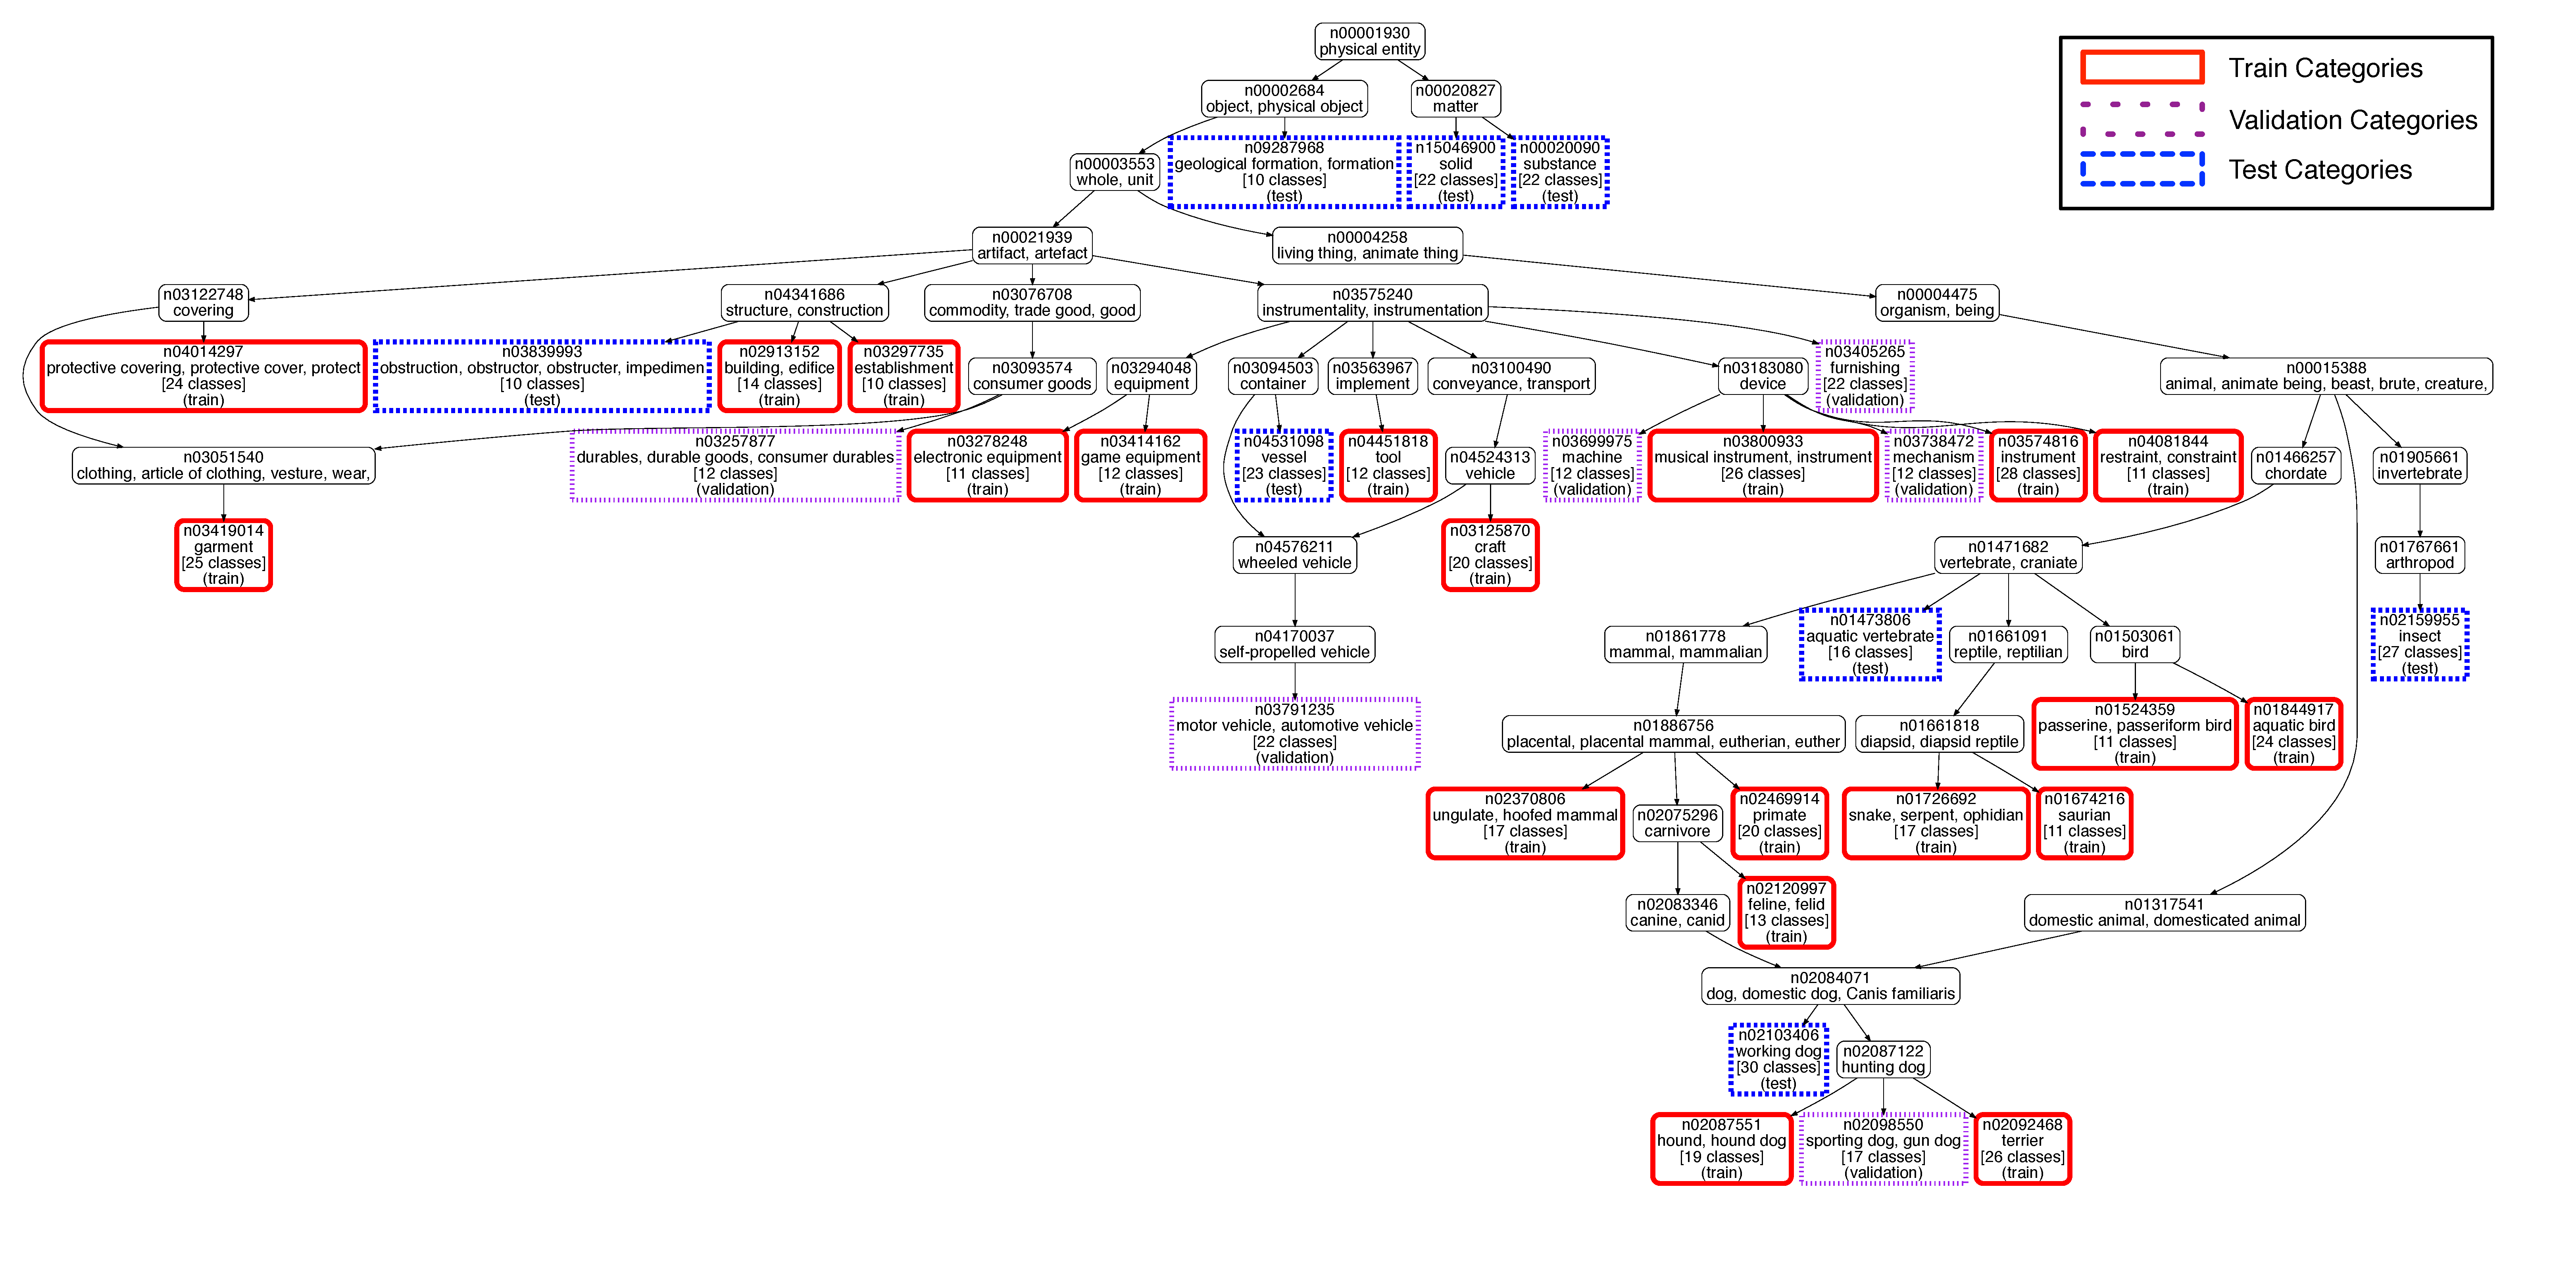
\includegraphics[width=\textwidth]{figures/hierarchy_legend_val.pdf}
    \caption{Hierarchy of \textit{tiered}Imagenet categories. Training categories are highlighted in red and test categories in blue. Each category indicates the number of associated classes from ILSVRC-12. Best viewed zoomed-in on electronic version.}
    \label{fig:tiered_hierarchy}
\end{sidewaysfigure}
\fi

\section{Extra Experimental Results}
\subsection{Few-shot classification baselines}
We provide baseline results on few-shot classification using 1-nearest neighbor and logistic
regression with either pixel inputs or CNN features. Compared with the baselines, Regular ProtoNet
performs significantly better on all three few-shot classification datasets.

\begin{table}[t]
    \centering
    \resizebox{\textwidth}{!}{
    \begin{small}
    \begin{tabular}{l|c|c|c|c|c}
                 & Omniglot            & \multicolumn{2}{c|}{\textit{mini}ImageNet}& \multicolumn{2}{c}{\textit{tiered}ImageNet}\\
    \cline{2-6}
    Models       & 1-shot              & 1-shot              & 5-shot              & 1-shot              & 5-shot               \\
    \hline
    \hline
    1-NN Pixel   & 40.39 $\pm$ 0.36    & 26.74 $\pm$ 0.48    & 31.43 $\pm$ 0.51    & 26.55 $\pm$ 0.50    & 30.79 $\pm$ 0.53     \\
    1-NN CNN rnd & 59.55 $\pm$ 0.46    & 24.03 $\pm$ 0.38    & 27.54 $\pm$ 0.42    & 25.49 $\pm$ 0.45    & 30.01 $\pm$ 0.47     \\
    1-NN CNN pre & 52.53 $\pm$ 0.51    & 32.90 $\pm$ 0.58    & 40.79 $\pm$ 0.76    & 32.76 $\pm$ 0.66    & 40.26 $\pm$ 0.67     \\
    \hline
    LR Pixel     & 49.15 $\pm$ 0.39    & 24.50 $\pm$ 0.41    & 33.33 $\pm$ 0.68    & 25.70 $\pm$ 0.46    & 36.30 $\pm$ 0.62     \\
    LR CNN rnd   & 57.80 $\pm$ 0.45    & 24.10 $\pm$ 0.50    & 28.40 $\pm$ 0.42    & 26.55 $\pm$ 0.48    & 32.51 $\pm$ 0.52     \\
    LR CNN pre   & 48.49 $\pm$ 0.47    & 30.28 $\pm$ 0.54    & 40.27 $\pm$ 0.59    & 34.52 $\pm$ 0.68    & 43.58 $\pm$ 0.72     \\
    \hline
    ProtoNet     &\tb{94.62 $\pm$ 0.09}&\tb{43.61 $\pm$ 0.27}&\tb{59.08 $\pm$ 0.22}&\tb{46.52 $\pm$ 0.32}& \tb{66.15 $\pm$ 0.34} 
    \end{tabular}
    \end{small}
    }
    \caption{Few-shot learning baseline results using labeled/unlabeled splits. Baselines either
    takes inputs directly from the pixel space or use a CNN to extract features. ``rnd'' denotes
    using a randomly initialized CNN, and ``pre'' denotes using a CNN that is pretrained for
    supervised classification for all training classes.}
    \label{tab:tieredImageNet}
\end{table}

\subsection{Number of unlabeled items}
Figure~\ref{fig:tnet_num_unlabel_text} shows test accuracy values with different number of unlabeled items during test time. Figure~\ref{fig:histo} shows our mask output value distribution of the masked soft k-means model on Omniglot. The mask values have a bi-modal distribution, corresponding to distractor and non-distractor items.
\begin{figure}
    \centering
    \iflatexml
    \includegraphics[width=6\textwidth]{figures/tnet_num_unlabel_text.png}
    \else
    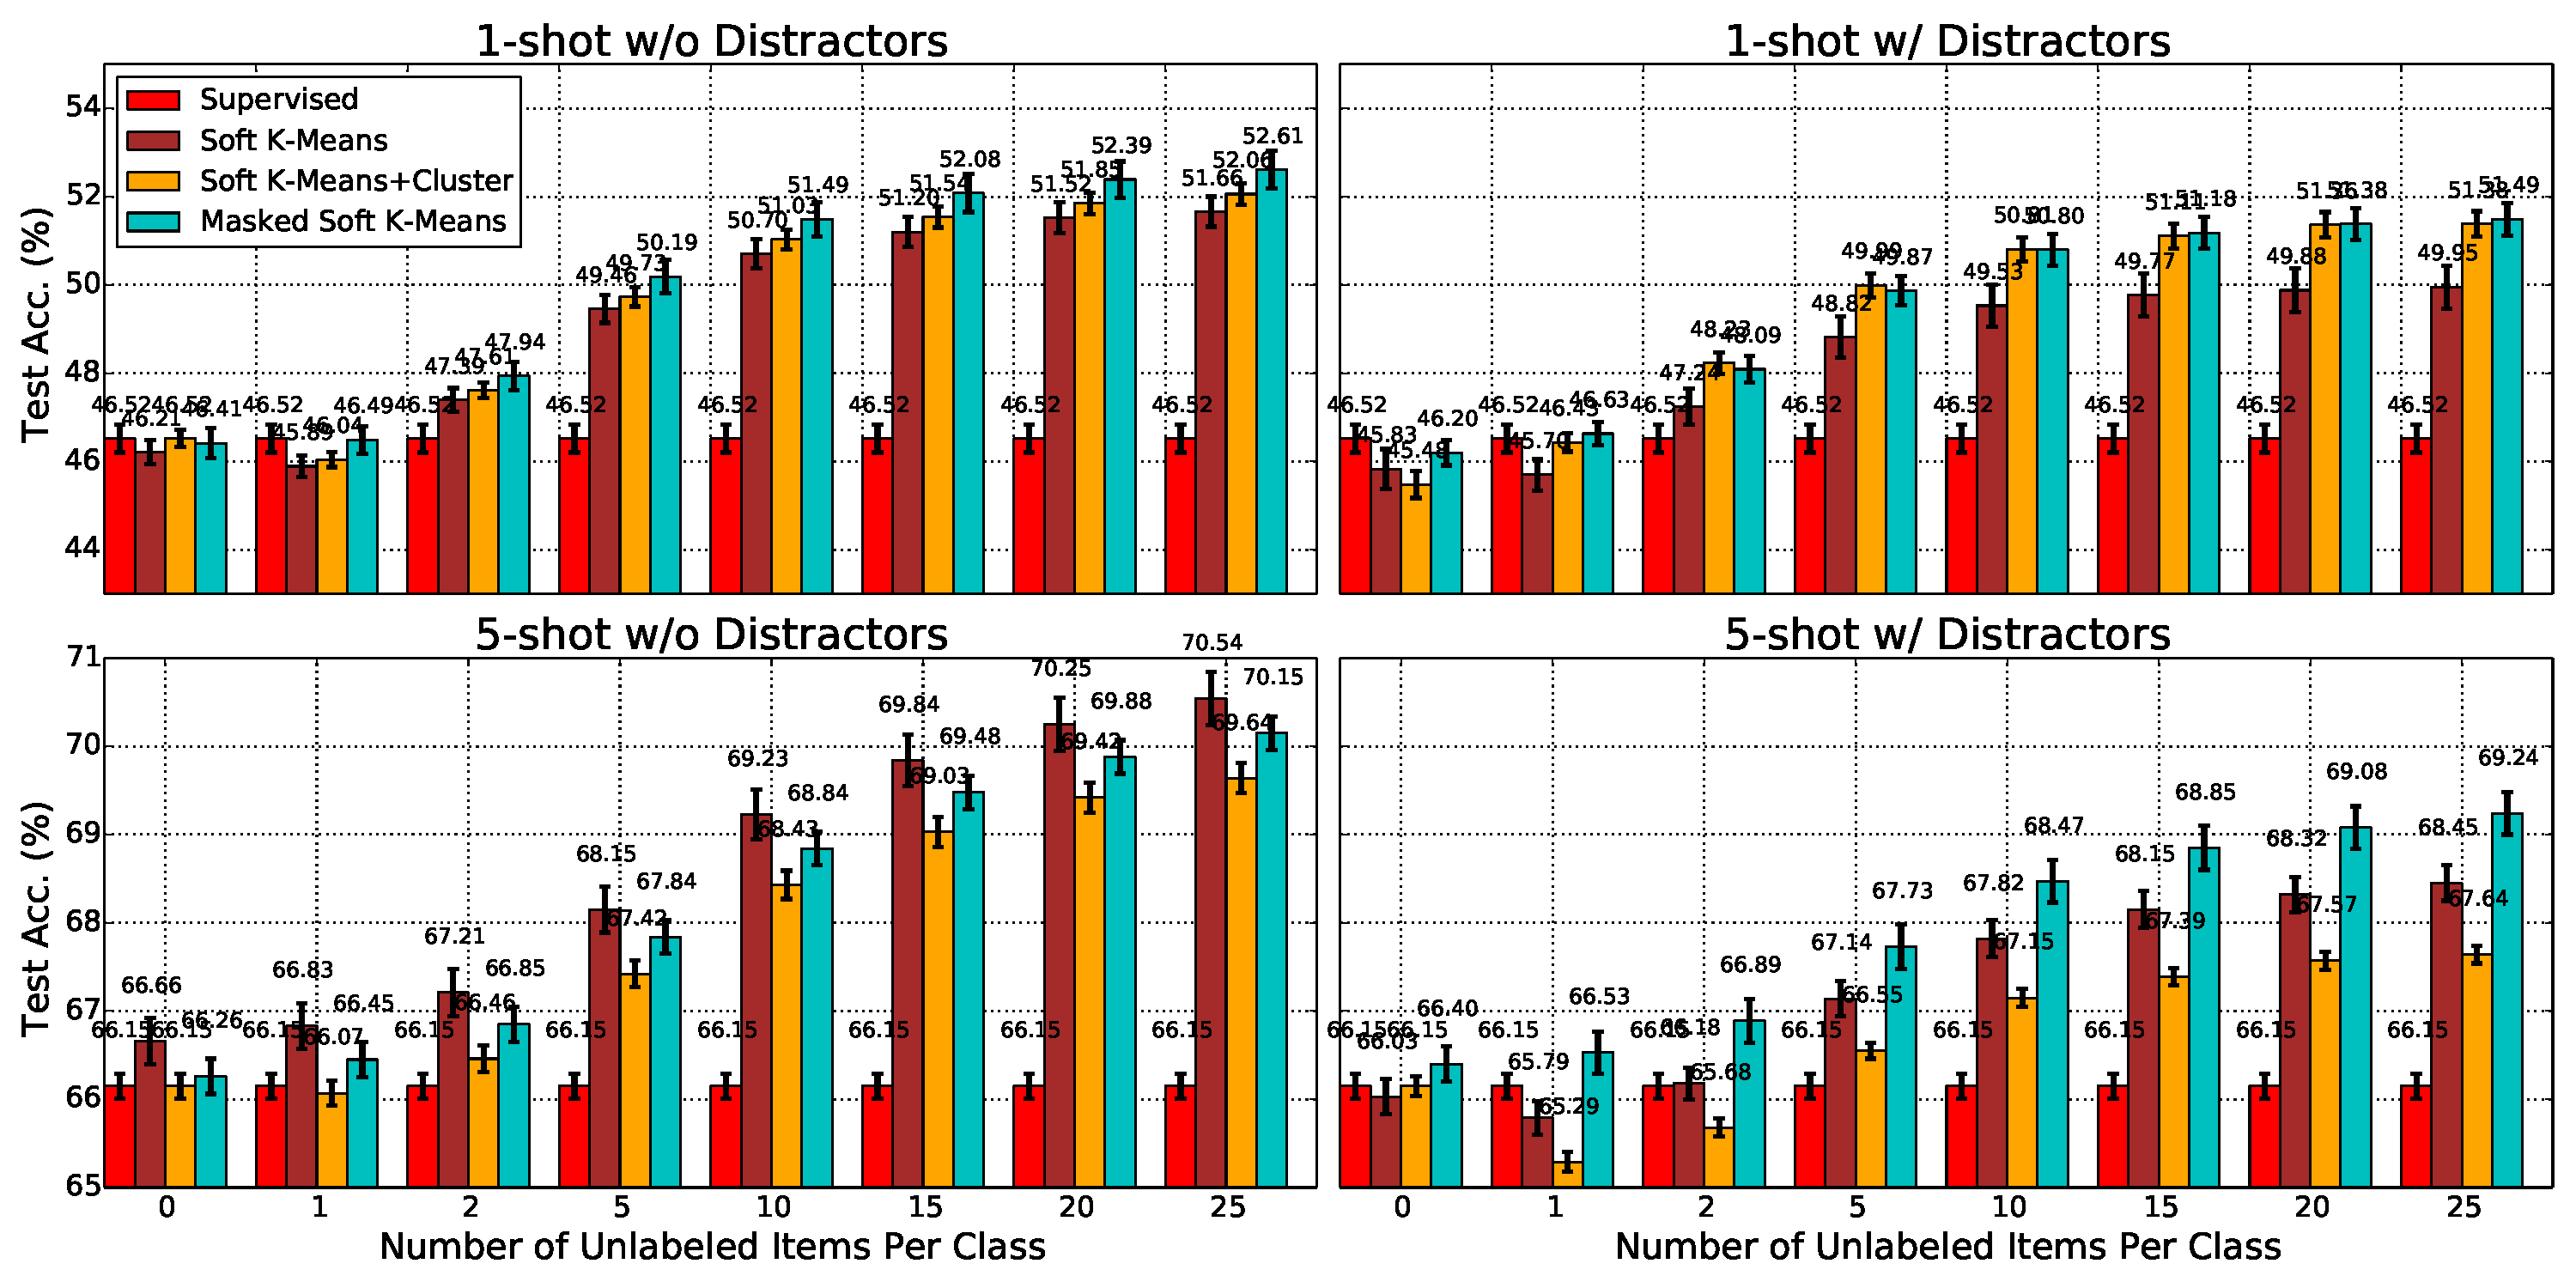
\includegraphics[width=\textwidth]{figures/tnet_num_unlabel_text.pdf}
    \fi
    \caption{Model Performance on \textit{tiered}ImageNet with different number of unlabeled items during test time. We include test accuracy numbers in this chart.}
    \label{fig:tnet_num_unlabel_text}
\end{figure}

\begin{figure}
    \centering
    \iflatexml
    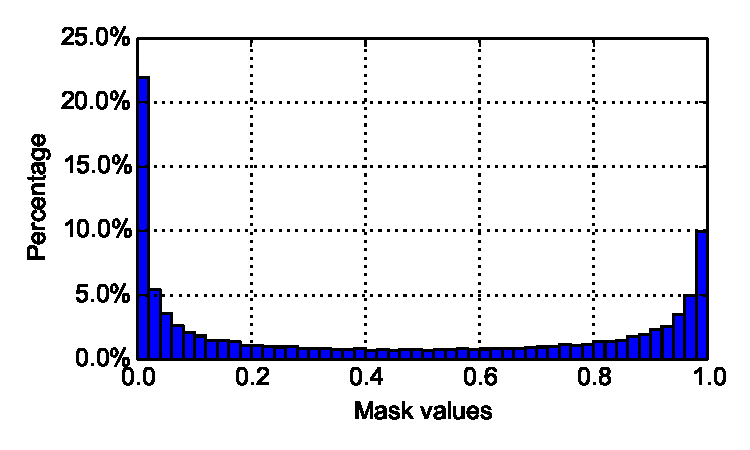
\includegraphics[width=4\textwidth]{figures/mask_histo_omniglot_refinement.pdf}
    \else
    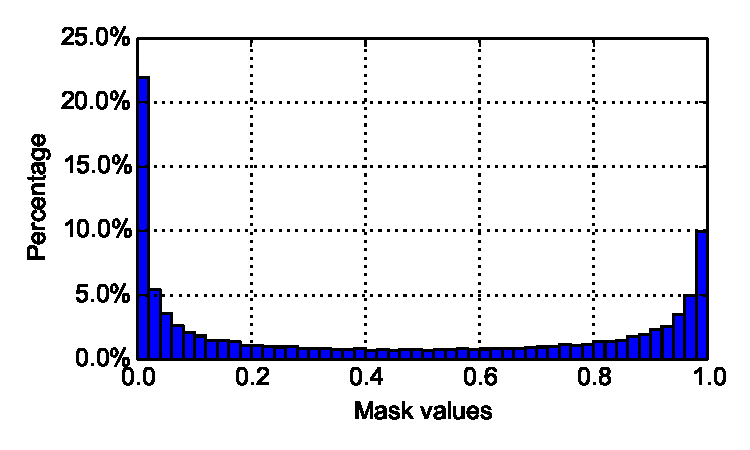
\includegraphics[width=0.7\textwidth]{figures/mask_histo_omniglot_refinement.pdf}
    \fi
    \caption{Mask values predicted by masked soft k-means on Omniglot.}
    \label{fig:histo}
\end{figure}

\section{Hyperparameter Details}
\label{sec:hyperparam}
For Omniglot, we adopted the best hyperparameter settings found for ordinary Prototypical Networks
in \cite{snell2017protonet}. In these settings, the learning rate was set to 1e-3, and cut in half
every $2$K updates starting at update 2K. We trained for a total of 20K updates. For
\textit{mini}Imagenet and \textit{tiered}ImageNet, we trained with a starting learning rate of 1e-3,
which we also decayed. We started the decay after 25K updates, and every 25K updates thereafter we
cut it in half. We trained for a total of 200K updates. We used ADAM \citep{kingma2014adam} for the
optimization of our models. For the MLP used in the Masked Soft $k$-Means model, we use a single
hidden layer with $20$ hidden units with a tanh non-linearity for all $3$ datasets. We did not tune
the hyparameters of this MLP so better performance may be attained with a more rigorous
hyperparameter search.
